\subsection{Systemsekvensdiagram}
Systemsekvensdiagram (figur \ref{fig:sysSekdia}) illustrere sekvensen af metodekald for at spille spillet. Sekvensdiagrammet viser dog kun et enkelt system (hoveddelen) af spillet. For at udføre nogle af de metoder som bliver kaldt på "Game" bliver der brugt yderligere metoder fra andre klasser f.eks. "Logic"
\begin{figure}[H]
    \centering
    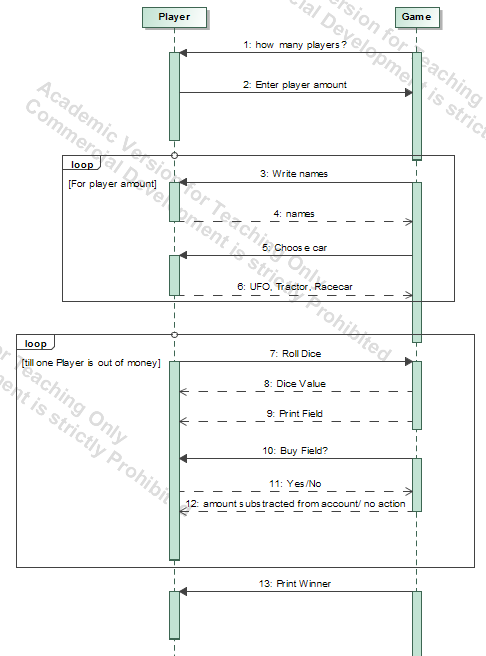
\includegraphics{sources/6_design/sekvensdiagram.PNG}
    \caption{Systemsekvensdiagram over kerne "loopet"}
    \label{fig:sysSekdia}
\end{figure}